\chapter{观测设计、误差预算和可行性计算}
\label{chap:18}

\begin{chapteropening}
观测设计从待测物理参数开始，再倒推望远镜和仪器设置。要测恒星角直径，就要知道 \(|V|^2(B,\lambda)\) 在哪些基线最敏感；要测强度相关，就要知道零延迟相关峰有多高、探测器会把它稀释到什么程度；要测偏振旋转或时间延迟，就要知道事件表里时间、频率和偏振标签的精度。强度干涉从 Hanbury Brown--Twiss 的 Sirius 实验、Narrabri 的 32 颗恒星角直径测量，到 VERITAS、MAGIC 和 photon-counting Vega 实验，使用的都是同一张可行性账本：光子率给出统计上限，相关 contrast 给出目标信号，基线、带宽、时间分辨率和校准误差决定这个信号能否留下来 \citep{1956Natur.178.1046H,1957RSPSA.242..300B,1958RSPSA.248..222B,1974MNRAS.167..121H,2006ApJ...649..399L,2020NatAs...4.1164A,2020MNRAS.491.1540A,2021MNRAS.506.1585Z}。
\end{chapteropening}

\section{从科学参数到事件表}

每个科学目标都对应一组待估计的物理参数 \(\boldsymbol\theta_{\rm phys}\)：恒星角直径、双星角分离、旋转星的扁率和位置角、谱线发射区半径、偏振角旋转、时延，或二阶相关峰的 contrast。仪器直接给出的是第 \ref{chap:01} 章式 \eqref{eq:event-row} 和第 \ref{chap:06} 章式 \eqref{eq:ch06-raw-event} 所描述的事件表，物理参数要从这些事件字段中估计。

观测设计从这些字段是否支撑目标参数开始：时间戳能否做 ns 相关，位置标签能否给出所需基线，波长和偏振标签是否保留，质量标记能否追踪天空背景、死时间、云量和时钟状态。若一开始只生成一张积分图像，后来想恢复 ns 时间相关或偏振相关，信息已经被平均掉；若保留事件表，后面可以投影成光变曲线、\(g^{(2)}(\tau)\)、\(|V|^2(B)\)、偏振角，或多波长 \(u,v\) 数据。

从参数到数据的关系可以写成
\begin{equation}
  \mathcal L(\boldsymbol\theta_{\rm phys})
  =
  P\!\left(d\,\middle|\,
  q_{\rm inst}(\boldsymbol\theta_{\rm phys}),
  {\bf c}_{\rm cal},
  {\bf b}_{\rm sky}
  \right).
  \label{eq:ch18-likelihood-chain}
\end{equation}
\begin{formulaexplain}[公式 (18.1) 解读]
\(\boldsymbol\theta_{\rm phys}\) 是要估计的物理参数，\(d\) 是事件表或其统计量。公式说明：物理参数先变成仪器可测量 \(q_{\rm inst}\)，再和校准项、背景项一起决定数据似然。
\end{formulaexplain}
\(\mathcal L\) 是似然；\(q_{\rm inst}\) 是仪器可测量，如 \(|V|^2\)、\(g^{(2)}-1\)、偏振 Stokes 量或到达时间残差；\({\bf c}_{\rm cal}\) 是校准参数，包括时间零点、滤光片通带、探测器效率和背景修正；\({\bf b}_{\rm sky}\) 是天光、月光、暗计数和宿主背景。实际 proposal 里，与其只写“我们会观测这颗星”，更有用的是写清这颗星的 \(m_B\)、\(\theta\)、可见窗口和模型先验会给出哪些 \(|V|^2\) 数据点，最终把 \(\theta\) 的误差压到多少。

角尺度先决定基线。空间频率、可见度和天空亮度的 Fourier 关系在第 \ref{chap:05} 章式 \eqref{eq:ch05-uv} 和 \eqref{eq:ch05-vcz} 中给出；观测设计直接用它的物理含义：振幅干涉测 \(V\) 的幅度和相位，强度干涉在热光近似下测 \(|V|^2\)。因此观测申请需要写清目标角尺度落在第几 lobe、需要哪些投影基线和位置角，以及相位缺失是否会导致模型退化 \citep{2003RPPh...66..789M,2009A&A...507.1719F,2012NewAR..56..143D,2014MNRAS.437..798M,2022MNRAS.512.1722K}。

粗略分辨率可用
\begin{equation}
  B
  \sim
  \frac{\lambda}{\theta}
  =
  86\,{\rm m}
  \left(\frac{\lambda}{416\,{\rm nm}}\right)
  \left(\frac{1\,{\rm mas}}{\theta}\right).
  \label{eq:ch18-baseline-scale}
\end{equation}
\begin{formulaexplain}[公式 (18.2) 解读]
\(B\) 是所需基线，\(\lambda\) 是观测波长，\(\theta\) 是目标角尺度。这个量级式把“要分辨多小”直接换成“需要多长基线”。
\end{formulaexplain}
\(\theta=2\,{\rm mas}\) 的热星在 416 nm 只需 \(\sim43\,{\rm m}\) 就开始被解析；\(\theta=0.5\,{\rm mas}\) 需要 \(\sim170\,{\rm m}\)；\(\theta=0.1\,{\rm mas}\) 进入 \(\sim860\,{\rm m}\) 级。Narrabri 的最大基线约 188 m，因此最擅长亮而热、角直径在几十分之一到几 mas 的恒星；CTA 型 km 阵列把空间频率推进到几十微角秒量级，但目标还要有足够光子率 \citep{1974MNRAS.167..121H,2006ApJ...649..399L,2010SPIE.7734E..1TJ,2013APh....43..331D}。

\section{光子率、带宽和相干稀释怎样决定可检性}

光子率从星等开始。AB 星等先换成谱流量密度：
\begin{equation}
  F_\nu=3631\,{\rm Jy}\,10^{-0.4m_{\rm AB}}.
  \label{eq:ch18-ab-flux}
\end{equation}
\begin{formulaexplain}[公式 (18.3) 解读]
\(m_{\rm AB}\) 是 AB 星等，\(F_\nu\) 是谱流量密度。星等每增加 5 等，\(F_\nu\) 下降 100 倍，因此光子率和相关信号也迅速变难。
\end{formulaexplain}
然后用第 \ref{chap:01} 章式 \eqref{eq:photon-rate} 把能量流量换成光子率。代入 550 nm、10 nm 通带和 \(\eta=0.25\)，一台 12 m 望远镜对 \(m_{\rm AB}=5\) 的源给出 \(R_\gamma\simeq2.8\times10^8\,{\rm s^{-1}}\)，对 \(m_{\rm AB}=8\) 给出 \(1.8\times10^7\,{\rm s^{-1}}\)。17 m MAGIC 级口径在同样假设下约为 \(5.7\times10^8\,{\rm s^{-1}}\) 和 \(3.6\times10^7\,{\rm s^{-1}}\)。这些数还不是可用相关事件率；它们会被空间模式、偏振、滤光片角入射、死时间、数据质量切片和背景修正继续削减 \citep{2006ApJ...649..399L,2020MNRAS.491.1540A,2021MNRAS.506.1585Z,2024MNRAS.529.4387A}。

\begin{figure}[tbp]
\centering
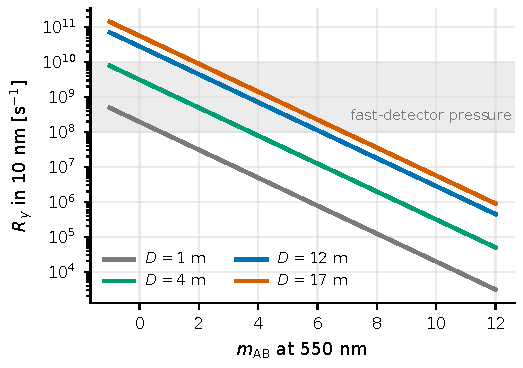
\includegraphics[width=0.86\linewidth]{figures/generated/chapter_18/ch18_photon_rate_magnitude.pdf}
\caption{AB 星等到窄带光子率的换算。曲线采用 550 nm、10 nm 通带和总效率 \(\eta=0.25\)。口径只线性改变收集面积，星等每增加 5 等会让光子率下降 100 倍；灰色区域标出 \(10^8\,{\rm s^{-1}}\) 以上的高速探测和数据吞吐压力。}
\label{fig:ch18-photon-rate}
\end{figure}

强度相关信号的高度由光学相干时间和电子响应共同决定。相干时间的带宽换算见第 \ref{chap:04} 章式 \eqref{eq:ch04-coherence-time}，热光峰的时间稀释见第 \ref{chap:04} 章式 \eqref{eq:ch04-contrast-dilution}。代入 VERITAS 常用的 416 nm、13 nm 通带，可得 \(\tau_c\simeq4.4\times10^{-14}\,{\rm s}\)；若探测器和电子链的等效时间宽度是 \(\Delta t=4\,{\rm ns}\)，未解析热光的零基线二阶相关峰自然落到几 \(10^{-6}\) 的量级。VERITAS 论文中测到的零基线归一化相关量 \(N_0\sim10^{-6}\) 处在同一量级；实际值还包含滤光片形状、探测器响应、偏振、背景和电子链修正 \citep{2020NatAs...4.1164A,2024ApJ...966...28A}。

\begin{figure}[tbp]
\centering
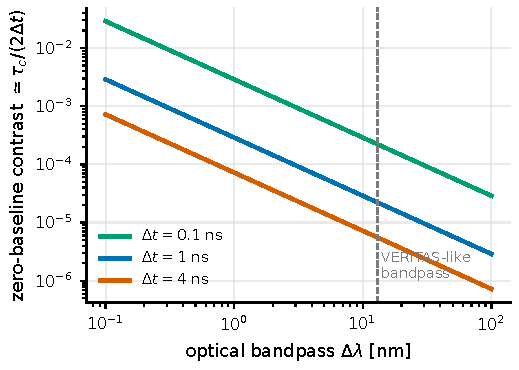
\includegraphics[width=0.86\linewidth]{figures/generated/chapter_18/ch18_coherence_dilution.pdf}
\caption{通带越宽，光学相干时间越短；电子时间分辨率越慢，零延迟相关峰越被稀释。416 nm、13 nm、4 ns 的组合给出几 \(10^{-6}\) 的 contrast，因此相关峰要靠长时间平均和严格校准才能从噪声中浮现。}
\label{fig:ch18-coherence-dilution}
\end{figure}

光学通带并不按单调方式改善 SNR。对理想热光强度干涉，若电子带宽远小于光学带宽，SNR 对光学通带宽度的一阶依赖会近似抵消：窄带减少光子数，但增加相干时间；宽带增加光子数，但降低每个时间 bin 的相关 contrast。真实仪器仍然关心滤光片，因为 PMT 或 SPAD 电流、天空背景、滤光片角入射和谱线科学目标都会改变可用信号。MAGIC 的低 \(f/D\simeq1\) 光束会让干涉滤光片在不同入射角下中心波长移动，实际通带比平行光测量更宽、更偏蓝；这会降低相关峰形状和 SNR，需要用光学模型和实验标定一起处理 \citep{2020MNRAS.491.1540A,2024MNRAS.529.4387A,2021MNRAS.506.1585Z}。

\section{强度相关的 SNR 怎样做第一轮估算}

双望远镜强度干涉的经典 SNR 标度已在式 \eqref{eq:ch05-snr} 中给出。设计阶段直接把目标星等、望远镜面积、总效率、电子带宽、积分时间和目标基线上的 \(|V|^2\) 代入该式即可。LeBohec 和 Holder 用 \(A=100\,{\rm m^2}\)、\(\alpha=0.3\)、\(\Delta f=1\,{\rm GHz}\)、\(T=5\,{\rm h}\)、\(|V|^2=0.5\) 得到 \(m_V\simeq6.7\) 的 \(5\sigma\) 量级估算；同样条件下 \(m_V=5\) 可达到二十以上的 SNR，而 \(m_V=9\) 只剩亚 sigma \citep{2006ApJ...649..399L,2008AIPC..984..205L,2012NewAR..56..143D}。

\begin{figure}[tbp]
\centering
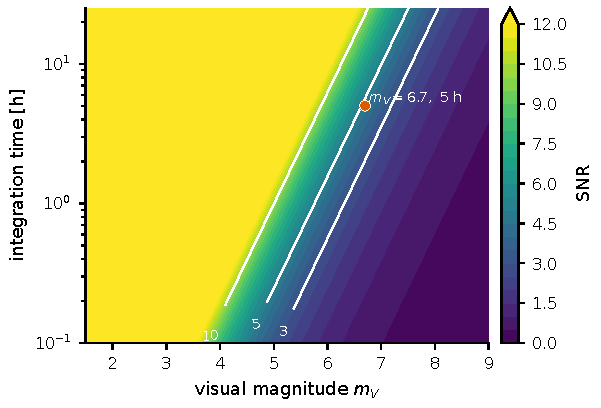
\includegraphics[width=0.90\linewidth]{figures/generated/chapter_18/ch18_snr_heatmap.pdf}
\caption{强度干涉 SNR 对星等和积分时间的依赖。图中采用 \(A=100\,{\rm m^2}\)、\(\alpha=0.3\)、\(\Delta f=1\,{\rm GHz}\)、\(|V|^2=0.5\)；橙点对应 LeBohec--Holder 估算中 \(m_V\simeq6.7\)、5 h 约 \(5\sigma\) 的位置。}
\label{fig:ch18-snr}
\end{figure}

式 \eqref{eq:ch05-snr} 只适合第一轮估算。真实数据里的 \(T\) 指通过质量切片后的有效 live time；\(\Delta f\) 指光学脉冲、PMT 或 SPAD 响应、线缆、放大器、digitizer 和软件相关共同形成的等效带宽；\(|V|^2\) 还会随目标高度和时角改变。VERITAS 的四台 12 m IACT 可同时给六条基线，采用 416 nm、\(\sim13\) nm 的滤光片和 4 ns 采样，每小时生成约 3.5 TB 原始数据；MAGIC 的两台 17 m 望远镜使用中央 PMT 和窄带滤光片，早期演示报告了比 Narrabri 约高一个数量级的灵敏度。Vega photon-counting 实验则展示了另一路线：用 SPAD 与软件相关在零基线得到 \(\langle g^{(2)}\rangle=1.0034\pm0.0008\)，在 \(\sim2\) km 投影基线上未检出相关，符合 Vega 约 3.3 mas 角直径已经被完全解析的预期 \citep{2020NatAs...4.1164A,2020MNRAS.491.1540A,2021MNRAS.506.1585Z,2024MNRAS.529.4387A}。

多基线同时增加数据量和几何信息。\(N\) 台望远镜给出 \(N(N-1)/2\) 条同时基线；4 台只有 6 条，60 台已有 1770 条。不同基线是在不同 \(u,v\) 点采样源结构，并非简单重复测量同一个数。若科学目标是一个均匀圆盘角直径，几条合适基线已经有用；若目标是快速旋转星的扁率、双星、盘风或非轴对称谱线发射区，就需要位置角覆盖。CTA 布局研究反复指出，长基线解析小尺度，但会丢掉整体形状；短基线测到总尺寸，却看不到高空间频率。覆盖 \(0.1-3\,{\rm mas}\) 的热星结构时，30--2000 m 的基线范围比单一最长基线更重要 \citep{2010SPIE.7734E..1CN,2010SPIE.7734E..1TJ,2012MNRAS.419..172N,2012MNRAS.424.1006N,2013MNRAS.430.3187R}。

\section{基线选择怎样变成参数灵敏度}

均匀圆盘是最常用的第一模型，其可见度和第一零点已在第 \ref{chap:05} 章式 \eqref{eq:ch05-uniform-disk} 和 \eqref{eq:ch05-first-null} 中给出。基线选择直接决定角直径信息量：若所有基线都在 \(|V|^2\simeq1\) 的平台上，不同 \(\theta\) 的曲线几乎重合；若只观测零点之后的极低可见度，相关峰又会接近噪声底。通常第一 lobe 下降区和第一零点附近给出最大的直径信息；limb darkening、快速自转和伴星会把曲线形状改掉，因此可行性计算要同时画目标模型的 \(|V|^2\) 和 \(\partial |V|^2/\partial\theta\) \citep{2003RPPh...66..789M,2020NatAs...4.1164A,2024ApJ...966...28A,2025ApJ...995..191A}。

\begin{figure}[tbp]
\centering
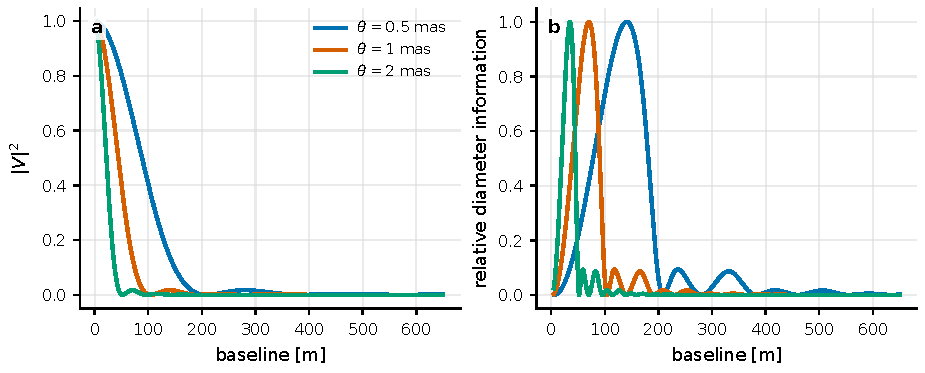
\includegraphics[width=0.94\linewidth]{figures/generated/chapter_18/ch18_visibility_fisher.pdf}
\caption{均匀圆盘的 \(|V|^2\) 曲线和直径灵敏度。416 nm 下，2 mas、1 mas 和 0.5 mas 目标的下降区分别落在几十米、百米和几百米基线；右图显示直径信息主要来自曲线斜率大的基线，短基线平台 \(|V|^2\simeq1\) 对直径不敏感。}
\label{fig:ch18-visibility-fisher}
\end{figure}

更一般的 Fisher 信息形式见第 \ref{chap:07} 章式 \eqref{eq:ch07-fisher} 和强度干涉专用的第 \ref{chap:08} 章式 \eqref{eq:ch08-sii-fisher}。在观测排程里，它的含义很直接：\(\mu_i\) 可以是 \(|V|^2\)、\(g^{(2)}\) 峰面积、偏振角或延迟；\(\sigma_i\) 应包含统计噪声和系统项。若某个基线的误差很小但导数几乎为零，它对目标参数几乎没有贡献；若导数大但 \(|V|^2\) 太低导致峰不可检出，也不能单独撑起结果。快速旋转星 \(\gamma\) Cas 的 VERITAS-SII 观测就是位置角覆盖的例子：不同投影基线采样不同方向的 \(|V|^2\)，从而约束扁率和长轴方向，单个等效圆盘直径不够描述这个目标 \citep{2025ApJ...995..191A,2024ApJ...966...28A}。

\begin{figure}[tbp]
\centering
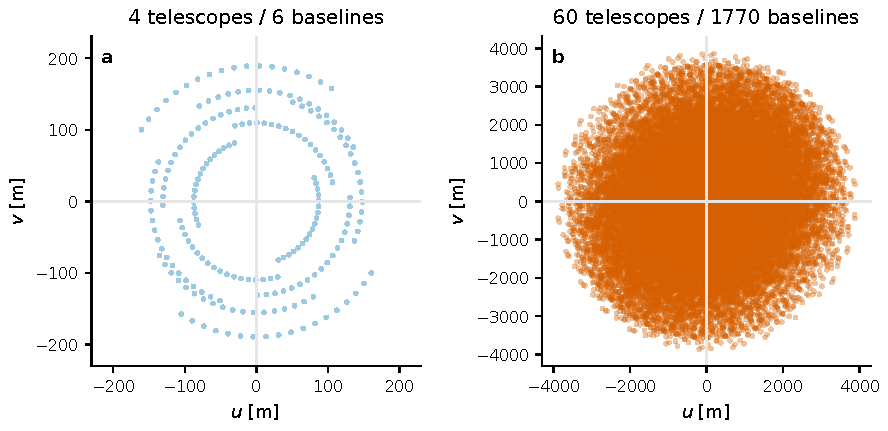
\includegraphics[width=0.94\linewidth]{figures/generated/chapter_18/ch18_uv_coverage.pdf}
\caption{阵列规模怎样改变 \(u,v\) 采样。左图是四台望远镜的示意覆盖，六条基线随时角旋转后仍较稀疏；右图是多望远镜 CTA 型阵列的示意覆盖，短基线、中等基线和长基线同时存在。密集覆盖不自动等于高 SNR，但它决定非轴对称目标能否被稳定拟合或重建。}
\label{fig:ch18-uv-coverage}
\end{figure}

波长也参与基线选择。同一物理基线在 416 nm 的空间频率比 800 nm 高约 1.9 倍；蓝端分辨率更高，但大气透过、镜面反射、探测量子效率和滤光片角入射更难。谱线观测还要考虑线通量而非宽带星等。对热星和 Be 星，H\(\alpha\)、He 或金属线可能来自比连续谱更大的发射区；窄带可以把几何结构和速度通道分开，但每个通道的事件率、滤光片泄漏和背景都要重新计算 \citep{2010SPIE.7734E..0AD,2012NewAR..56..143D,2021MNRAS.506.1585Z,2024MNRAS.529.4387A}。

\section{背景、校准和质量切片怎样进入系统误差}

背景不相关时，它主要稀释相关峰；两通道背景稀释因子的定义和假设已经在第 \ref{chap:06} 章式 \eqref{eq:ch06-background-dilution} 中给出。观测设计需要把这个修正落实到同一通道、同一增益状态和相近时间的背景测量上。VERITAS 的 \(\beta\) UMa 分析用目标附近 \(0.5^\circ\) 的 off runs 估计非星光电流，典型 off-source 强度约为 on-source 的 \(3\%\)，因此对半径拟合影响很小；明月、云、雾、城市光或 detector afterpulsing 会让这个近似变差，需要单独质量切片 \citep{2024ApJ...966...28A,2025ApJ...995..191A}。

\begin{figure}[tbp]
\centering
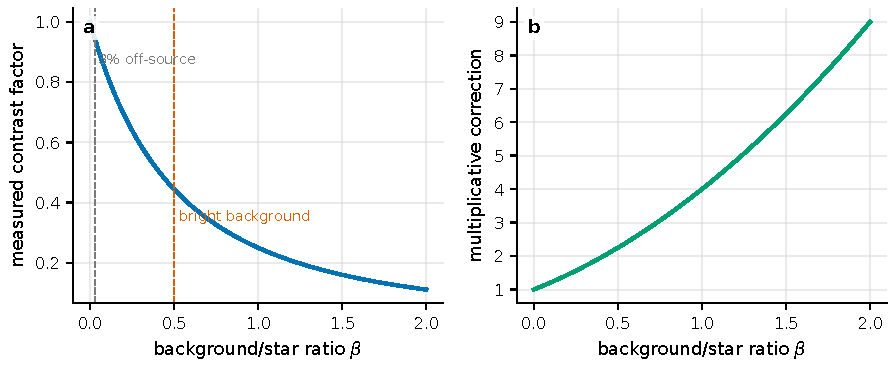
\includegraphics[width=0.94\linewidth]{figures/generated/chapter_18/ch18_background_dilution.pdf}
\caption{不相关背景对相关峰的稀释。若两端背景/星光比相同，观测 contrast 按 \((1+\beta)^{-2}\) 下降；\(\beta=0.03\) 只造成几个百分点修正，\(\beta=0.5\) 已把峰压到原来的约 44\%。右图给出反向修正因子，修正越大，对背景估计误差越敏感。}
\label{fig:ch18-background-dilution}
\end{figure}

时间校准是强度干涉和 photon counting 的共同硬件边界。相关峰宽度通常是几 ns；如果不同望远镜的相对延迟模型错了 1 ns，峰会被摊宽或移出拟合窗口。Vega photon-counting 实验中，零基线子孔径相对时间精度约 \(100\,{\rm ps}\)，两台望远镜之间还要处理光行时、仪器延迟、GPS 或 rubidium clock 漂移以及光纤色散，最终用 \(\sim400\,{\rm ps}\) time bin 做相关；他们指出多望远镜实现需要约 ns 级同步才能把观测时间保持在小时量级。VERITAS-SII 用 White Rabbit 10 MHz 时钟分发和 4 ns 采样，仍要在每个 run 中跟踪光程延迟随时角的变化，并处理 run-to-run 的峰位置变化 \citep{2021MNRAS.506.1585Z,2024ApJ...966...28A}。

校准星的选择要和科学目标同等认真。一个理想校准星应有已知角直径、稳定光度、接近目标的天空位置、相似颜色和足够高的光子率。若目标是 0.5 mas 热星，而校准星直径不确定到 \(5\%\)，最终直径误差很容易被校准项主导。现代强度干涉观测常把已知角直径热星作为 reference，先检查零基线归一化、滤光片响应和 \(|V|^2(B)\) 形状，再观测未知目标。MAGIC 2024 年的性能论文用多颗参考星验证系统，再给出新恒星角直径；VERITAS 的 \(\beta\) UMa 和 \(\gamma\) Cas 观测则展示了同一套系统从圆盘直径走向扁率和位置角测量 \citep{2024MNRAS.529.4387A,2024ApJ...966...28A,2025ApJ...995..191A}。

\section{误差预算怎样写进观测申请}

最终误差需要拆成统计项和系统项。对一个拟合参数 \(\theta\)，常用的误差预算为
\begin{equation}
  \sigma_\theta^2
  =
  \sigma_{\rm stat}^2
  +
  \sigma_{\rm bg}^2
  +
  \sigma_{\rm time}^2
  +
  \sigma_{\rm cal}^2
  +
  \sigma_{\rm model}^2 .
  \label{eq:ch18-error-budget}
\end{equation}
\begin{formulaexplain}[公式 (18.4) 解读]
\(\sigma_\theta\) 是目标参数的总误差，右边把统计、背景、时间、校准和模型误差分开。它提醒观测计划不能只报 SNR，还要说明误差平台来自哪里。
\end{formulaexplain}
\(\sigma_{\rm stat}\) 来自有限符合计数或相关峰拟合；\(\sigma_{\rm bg}\) 来自 off-source 背景插值和暗电流；\(\sigma_{\rm time}\) 来自时钟、几何延迟、采样和峰形；\(\sigma_{\rm cal}\) 来自校准星、throughput、滤光片和偏振；\(\sigma_{\rm model}\) 来自源模型，例如把快速旋转星当成圆盘、把谱线盘当成高斯、或忽略伴星。统计误差通常随 \(T^{-1/2}\) 下降，其他项常形成平台；当平台已经高于目标精度，继续加积分时间不会解决问题。

\begin{figure}[tbp]
\centering
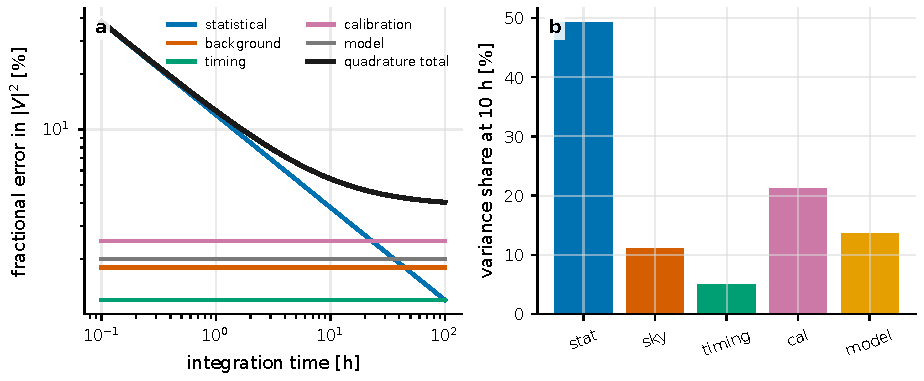
\includegraphics[width=0.94\linewidth]{figures/generated/chapter_18/ch18_error_budget.pdf}
\caption{误差预算中的统计项和系统项。左图显示统计误差随积分时间下降，但背景、时间、校准和模型项形成平台；右图把 10 h 时各项对总方差的贡献列出。观测申请应把每一项连接到可观测的校准数据，并给出总 SNR 之外的误差平台。}
\label{fig:ch18-error-budget}
\end{figure}

\begin{longtable}{p{0.18\linewidth}p{0.30\linewidth}p{0.42\linewidth}}
\toprule
量 & 常见范围 & 在计划中的用法 \\
\midrule
\(m_V,m_B\) & \(-1\) 到 \(9\) 等是当前 SII 的主战场 & 转成 \(n\) 或 \(R_\gamma\)，先判断目标是否过暗。 \\
\(A_{\rm eff}\) & \(1-250\,{\rm m^2}\) 每台望远镜 & 进入光子率和 SNR，镜面老化、遮挡和光纤耦合要算进效率。 \\
\(\Delta\lambda\) & \(0.1-30\,{\rm nm}\) & 决定相干时间、PMT 电流、天空背景和谱线选择。 \\
\(\Delta t\) & \(0.1-5\,{\rm ns}\) & 决定相关峰被稀释的程度和可用电子带宽。 \\
\(B_p\) & \(10-2000\,{\rm m}\) & 决定角尺度和 \(u,v\) 覆盖；短基线和长基线约束不同结构。 \\
\(\beta\) & \(0.01-1\) & 背景/星光比，决定 contrast 稀释和背景系统误差。 \\
\(\sigma_{\rm cal}\) & \(1-10\%\) 的可见度或直径量级 & 常成为长积分后的误差平台。 \\
\bottomrule
\end{longtable}

一份可执行的观测申请从目标参数写起，例如“测量 \(\gamma\) Cas 蓝光 photosphere 的长短轴比到 \(5\%\)”或“测量 1 mas A 型星的 limb-darkened 直径到 \(3\%\)”。目标描述随后给出星等、颜色、角直径估计、可见窗口，以及已有 CHARA/VLTI/Keck 或 Narrabri 数据。仪器部分要把望远镜数量、基线范围、滤光片中心波长和带宽、采样时间、同步方案、数据率和质量切片写清。

SNR 应按最有信息量的基线分别报告：统计精度来自式 \eqref{eq:ch05-snr}，背景修正来自式 \eqref{eq:ch06-background-dilution}，系统项则进入式 \eqref{eq:ch18-error-budget}。成功标准也要量化，例如至少三条基线在第一 lobe 下降区达到 \({\rm SNR}>5\)，校准星重复观测给出小于 \(3\%\) 的归一化漂移，off-source 背景修正小于总信号的 \(10\%\)。若长基线未检出，结果仍可给出角直径上限或排除过大的发射区；若校准平台过高，也能反推出仪器升级所需的时间同步、滤光片或背景控制指标。

这条估算链条同样适用于强度干涉之外的项目。振幅干涉、量子网络望远镜、CMB 偏振、FRB photon statistics 和实验室教学台架都需要同样的结构：事件率、模式数、响应函数、校准项、模型导数和误差预算。差别只在可观测量 \(\mu_i\) 的形式。科学案例排序也要沿用这个思路，把“科学价值”与“可观测性”分开评分，避免把漂亮目标和可执行目标混在一起 \citep{2010SPIE.7734E..0AD,2012MNRAS.419..172N,2012MNRAS.424.1006N,2013APh....43..331D,2014SPIE.9146E..0ZD,2017MNRAS.472.4126G,2022SPIE12183E..0DK,2024SPIE13095E..0IT,2026arXiv260212717K}。

